% Chapter Template

\chapter{TrustZone} % Main chapter title

\label{Chapter2} % Change X to a consecutive number; for referencing this chapter elsewhere, use \ref{ChapterX}

% 思路:
% 1. 介绍TrustZone
% 2. 介绍SANCTUARY
% 3. 小结。

%


%----------------------------------------------------------------------------------------
%	SECTION 1
%----------------------------------------------------------------------------------------

\section{Arm TrustZone}

\subsection{基本介绍} 
TrustZone是一种提高安全性能的硬件架构设计。
它提升了CPU,内存和其他部件的安全能力。
一个支持TrustZone的CPU处理器,可以在四种特权等级下执行指令(EL0-EL3)。
同时TrustZone通过硬件TrustedFirmware(TF)划分了普通世界(Normal World)和安全世界(Secure World)。
EL3拥有最高权限,也被称为monitor mode,可以通过运行ARM Trusted Firmware (TF) 来进行Normal World和Secure World之间的切换。
每个世界中都分别管理自己的地址空间和操作系统,
在Secure World中所有App都是运行在可信的操作系统(Trusted OS)上。
在Normal World中所有的App都运行在普通操作系统中。
EL2级别的指令是为每个世界中虚拟机提供的权限,EL1是操作系统内核权限,EL0是用户代码权限。


\begin{figure}
    \centering
    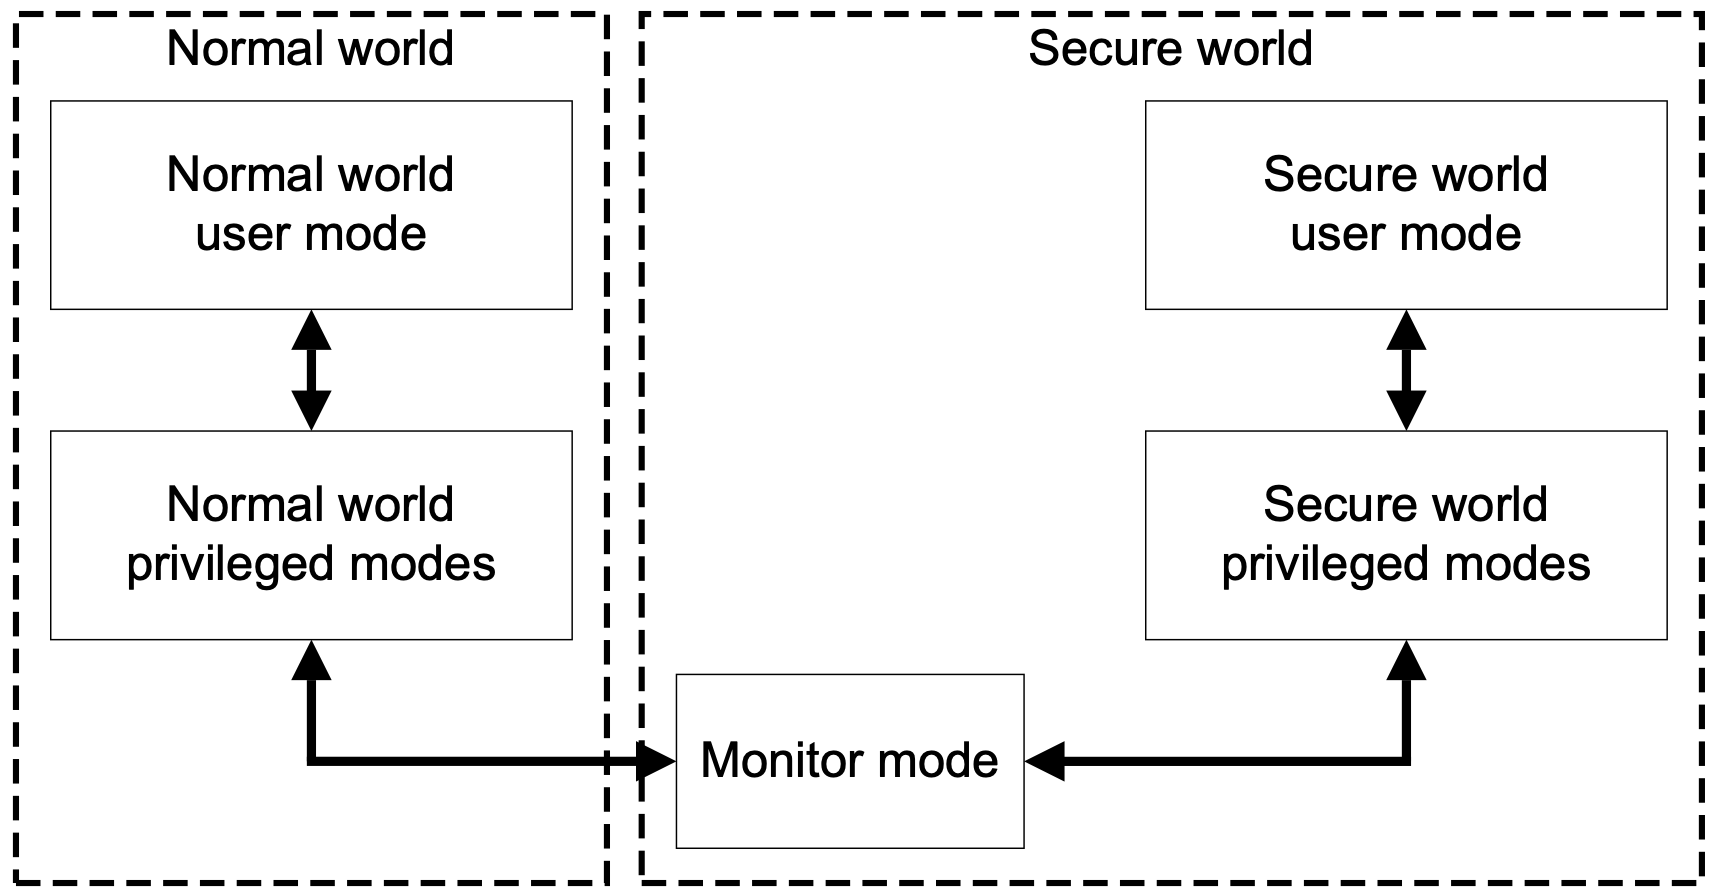
\includegraphics[scale=0.45]{Figures/trustzone/trustzone.png}
    \decoRule
    \caption{TrustZone基本权限设计}
    \label{fig:trustzone}
\end{figure}

(图~\ref{fig:trustzone})展示了TrustZone对Secure World和Normal World的划分,
每个CPU可以通过L3级别(monitor mode)的指令secure monitor call (smc)来进行
Secure World和Normal World之间的切换。图中展现了操作系统EL1和应用EL0两种权限,


\subsection {威胁模型} 
原始的TrustZone在威胁模型中作出如下假设:
\begin{itemize}
    \item
    TrustZone的安全模型认为Normal World中的App都是不可信的;
    \item
    在Normal World中运行的OS也是不可信的;
    \item 
    Trusted Firmware是可信的;
    \item
    Secure World中的App,操作系统和boot loader都是可信的。
\end{itemize}

\subsection{安全保证}
首先一个跑在ARM TrustZone的设备会从Secure World中启动,
在初始化完成之后会启动可信操作系统TOS,而boot loader会在执行TOS之前对其进行检查,
确保TOS没有被修改过,接着切换到Normal World启动普通操作系统。
按照这种顺序执行可以保证启动过程的安全,只要boot loader可信就可以保证TOS的完整性。
而在实际场景中终端运营商会通过加锁来防止boot loader被修改。

\begin{figure}
    \centering
    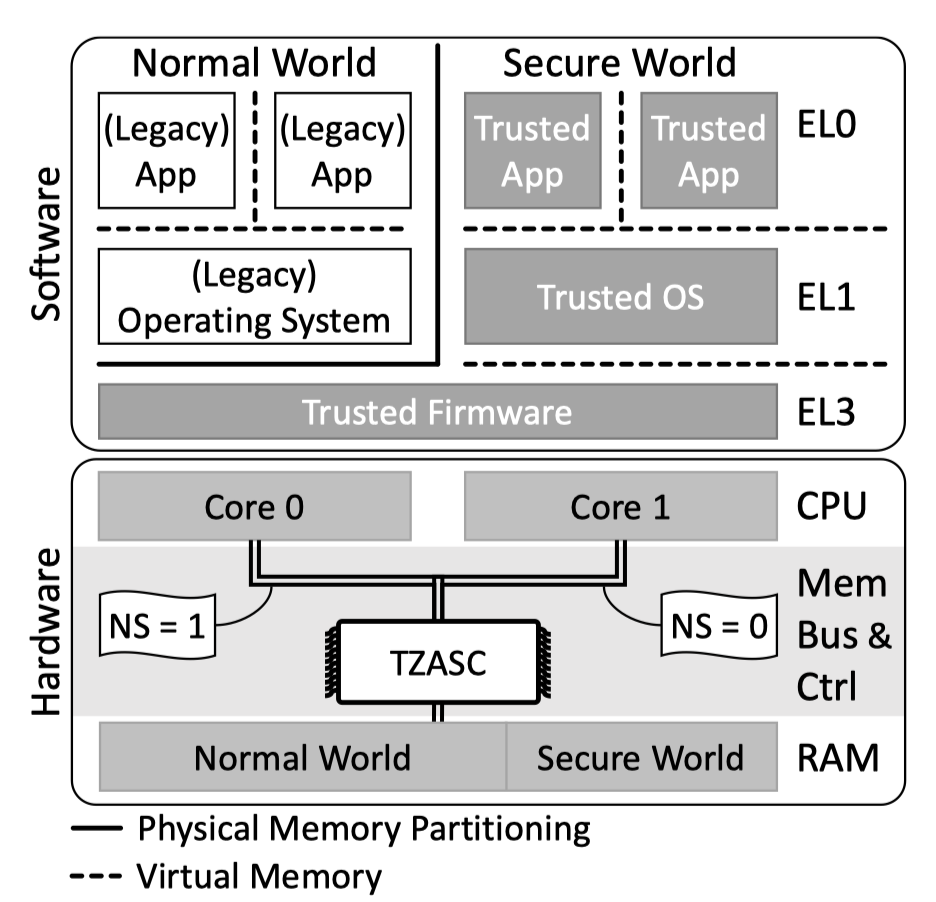
\includegraphics[scale=0.6]{Figures/trustzone/TZASC.png}
    \decoRule
    \caption{TrustZone的TZASC设计}
    \label{fig:tzasc}
\end{figure}
    
其次,TrustZone通过硬件层面上的隔离来防止Secure World中的App和OS被恶意代码攻击。
TrustZone直接将物理内存划分为两部分,其中一部分只能被Secure World访问。
这种物理上的强制隔离主要通过地址空间控制器TrustZone Address Space Controller(TZASC)
来实现。TZASC主要作用于总线和内存之间。
(图~\ref{fig:tzasc})展示了TrustZone Address Space Controller(TZASC)
的基本设计的最原始模式。最原始的TZASC只包含两种内存访问权限non-secure access(NS = 1)
和secure access(NS = 0)。
一个处于secure模式下的CPU可以访问non-secure和secure的内存,
而在non-secure模式下的CPU仅可以访问non-secure的内存。
TZASC现在已经有TZC-380,TZC-400等版本
较新的版本TZC-400,CPU,GPU,DMA等设备都会在硬件上被分配一个bus-master id,
每次访存操作都会附上这个id,这个id可以被用来分配固定物理内存和访问权限,以此做到
物理内存的隔离。
TZASC是使用这种机制来从空间上保证Secure World中的内存不会被其他CPU访问。



\subsection{不足}
传统的TrustZone存在下列不足:
\begin{itemize}
    \item
    在可信执行环境中,可信的应用(TA)之间的隔离程度较弱,
    一旦一个TA有恶意代码或被攻击,其他应用程序中的敏感数据也会被攻击。
    \item
    在Secure World中的TCB随着App的增多会不断扩展。
    \item 
    一旦黑客可以攻击到Secure World中,收益巨大,使的Secure World成为高价值的攻击目标。
    \item
    在TrustZone的设计中,一个带有敏感数据(需要被保护)的应用程序(Sensitive App)必须也是一个可以信任的应用程序(Trusted App),
    这样才能够放入Secure World中。
    一个应用程序成为可信应用程序需要运营商和软件开发者相互信任,
    同时需要做大量的检查工作。对于小的开发者来说,
    与vendor建立信任关系并且验证代码是一件费时费力的事情。
    对于vendor来说并不一定就能完全发现可信应用中的恶意代码或者可能被其他人利用的漏洞。
\end{itemize}


%----------------------------------------------------------------------------------------
%	SECTION 2
%----------------------------------------------------------------------------------------
\section{SANCTUARY}
\subsection{基本介绍}
\paragraph{模型改良}
SANCTUARY是在TrustZone的基础上为上面的不足提出了合理的解决方案。 
SANCTUARY区分了可信应用程序(Trusted App)和敏感应用程序(Sensitive App),
并把敏感应用程序列入可能有害的威胁模型中。
通在Normal World和Secure World之间设立一个新的区间Sanctuary,如(图~\ref{fig:sanctuary}),
来增加敏感应用程序之间的隔离性。
对于一个运行在Sanctuary中的Sensitive App,Sanctuary可以既保证它免于被入侵,
又可以防止他攻击其他敏感应用程序。
这种设计相比于原来的设计增加了隔离性,减小TCB,
同时一定程度上解决了运营商和应用程序开发者之间协调的问题。

\paragraph{隔离机制}
Sanctuary建立较强的隔离机制,空间上的隔离包括使用TZC-400内存访问控制器,
采用与TrustZone相似的方式强制隔离物理内存,Sanctuary的CPU只能访问自己的物理内存,
不能访问Secure World和Normal World中的内存对于每一个Sanctuary实例单独分配一个独立的CPU资源。
通过避免使用共享缓存,来防止独立内存数据的丢失。
时间上的隔离,包括每次都会从可信的固件(Trusted Firmware)中启动为Sanctuary分配的CPU,
在同一时刻内一个Sanctuary环境中只会运行一个应用程序(Sanctuary App),
并且在程序执行结束退出后,会清空其之前使用的内存和缓存。

\paragraph{安全服务}
由于在Sanctuary App执行之前会从没有保护的内存中加载数据。SANCTUARY需要做两种保护。
一种是要保证数据的可靠性,需要验证数据没有被修改过,另一方面SANCTUARY需要防止这些数据
被加载到以一个恶意的Sanctuary App中,因此Sanctuary App本身也需要被验证。对于上面两种
保护,Sanctuary提供了两种安全服务来进行保障。 一种是Remote attestation通过让Sanctuary App
与外部实体建立换一个安全的通道,Sanctuary App通过此通道向提供程序的第三方传输完整性测量数据,
以此保证数据的完整性。第二种是Sealing,这个机制给最初始的Sanctuary App分配一个key,这个
key根据Sanctuary App的哈希值计算得到。Sanctuary App在存储数据时通过这个密钥key进行加密,
读取数据时用这个key进行解密。这样被篡改的Sanctuary App的key会发生变化,因此不能解密得到
正确的数据

\begin{figure}
    \centering
    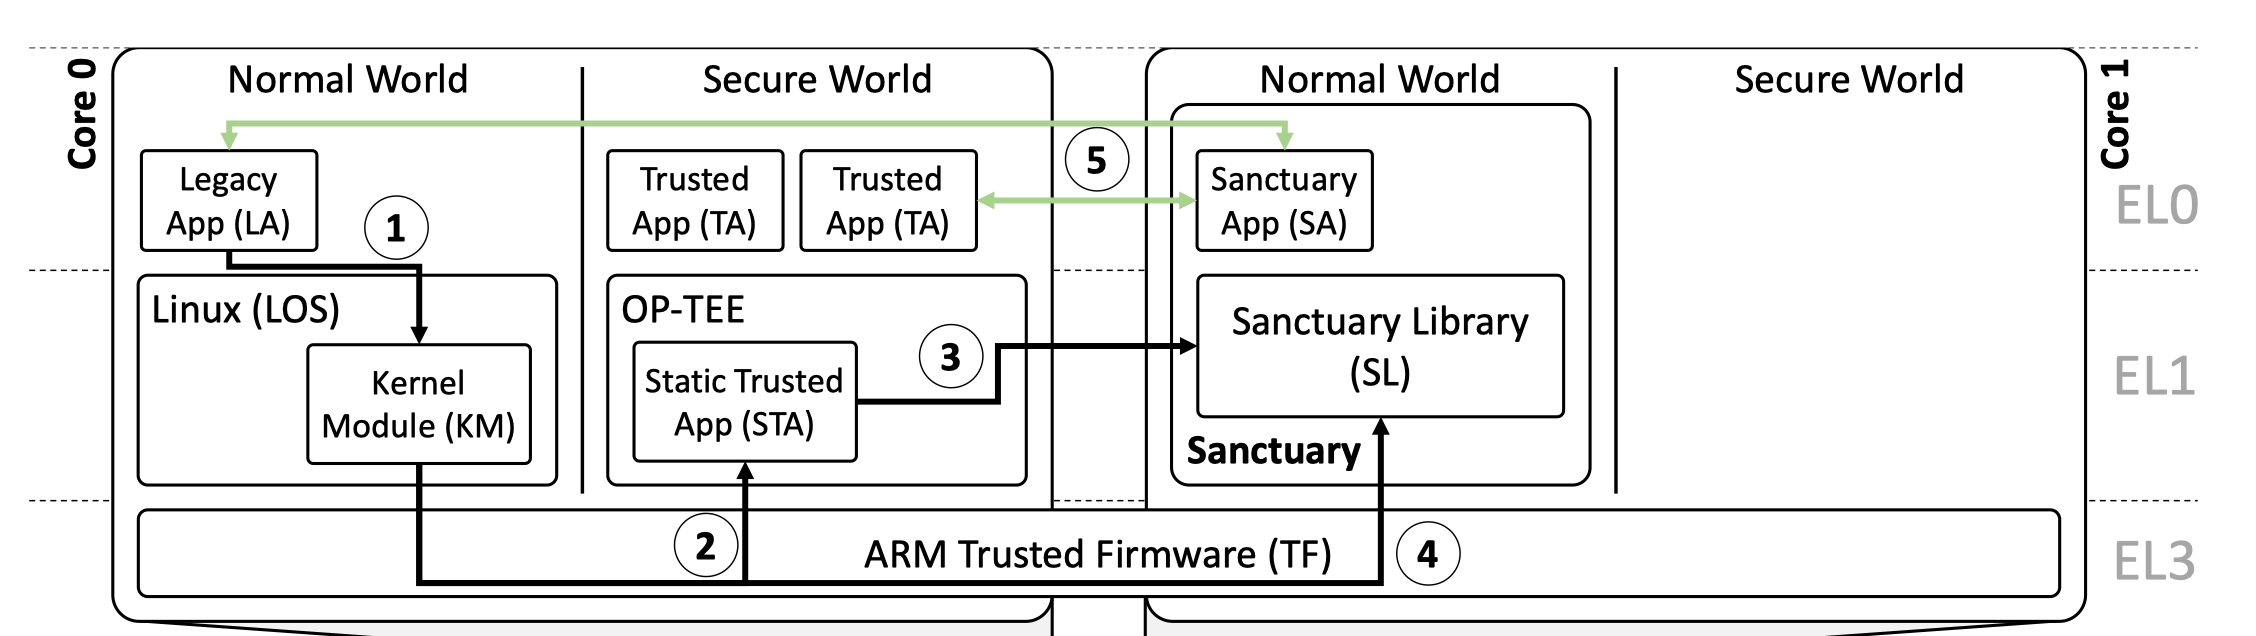
\includegraphics[scale=0.35]{Figures/trustzone/step.png}
    \decoRule
    \caption{Sanctuary 启动步骤}
    \label{fig:step}
\end{figure}

\paragraph{使用方式}
通常,当一个在Normal World中的App需要执行涉及敏感数据的代码时,会调用Normal World
中的Kernal Module(KM)创建一个Sanctuary进行执行。这其中包含五个步骤。如(图~\ref{fig:step})
\begin{itemize}
    \item
    1. 向KM提出执行的Sanctuary App的请求
    \item
    2. KM加载执行Sanctuary必要的运行数据包括Sanctuary library和Sanctuary App,并从
    服务Normal World的CPU中删掉一个,并交给Secure World中的一个专门负责创建相关
    的Trusted App(STA)来操作;
    \item 
    3. STA对Sanctuary App进行一些列的验证操作;
    \item
    4. 验证成功之后,创建Sanctuary实例,并启动;
    \item
    5. 启动后Sanctuary library可以执行敏感代码,并可以与LA和TA进行交流。
    \item
    同时攻击者不进行物理攻击。
\end{itemize}

\begin{figure}
    \centering
    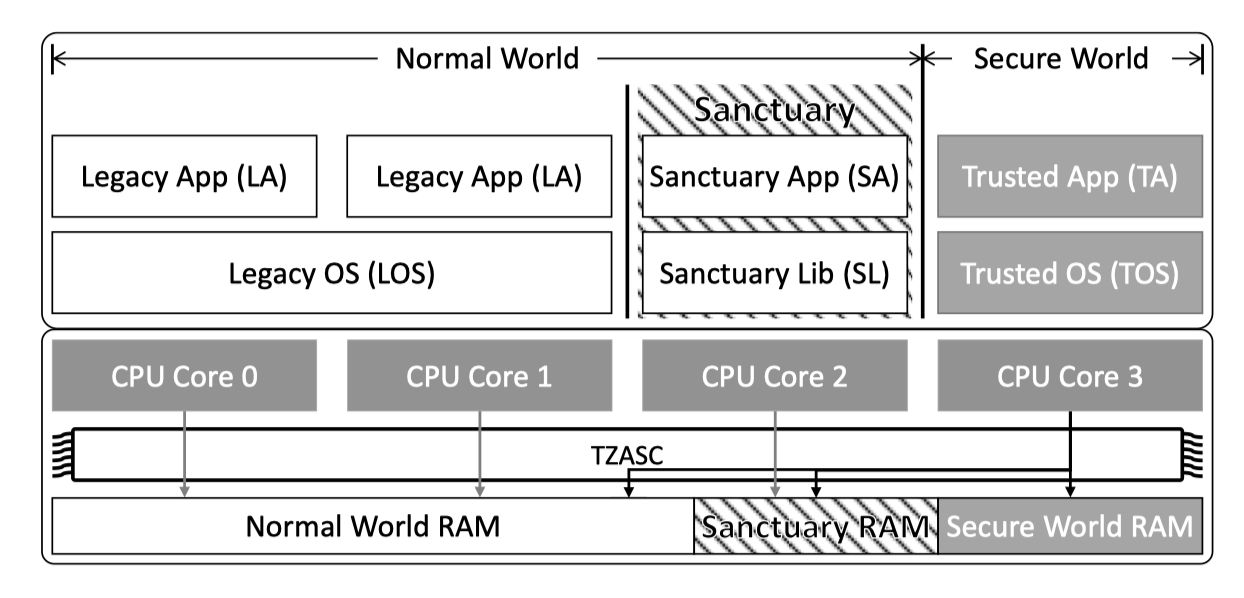
\includegraphics[scale=0.45]{Figures/trustzone/sancutary.png}
    \decoRule
    \caption{SANCTUARY结构图}
    \label{fig:sanctuary}
\end{figure}

\subsection{威胁模型}
SANCTUAR的威胁模型和TrustZone相比进行列继承,细化和延伸:
\begin{itemize}
    \item
    Normal World中的App都是不可信的;
    \item
    在Normal World中运行的OS也是不可信的;
    \item 
    运行在Sanctuary中的敏感应用程序(Sensitive App)也可能是具有恶意的;
    \item
    在Sanctuary假设基于TrustZone的Firmware是可信的;
    \item
    Secure World中的App,操作系统和boot loader都是可信的。
\end{itemize}

\subsection{安全保证}
为了满足威胁模型的要求,既需要保护Sanctuary App免遭攻击,有需要防止有恶意的
Sanctuary App攻击其他部分。接下来从可以攻击的各个角度来详细阐述它的安全保证。

\paragraph{二进制代码完整性}
Sanctuary Library和Sanctuary App的可执行数据都被存在未加密的Normal World的内存中,
SANCTUARY通过本地的验证和远程的验证(Remote attestation)本地验证通过SA最开始存储的
签名来验证,远程验证可以由开发者通过可信通道自己进行验证。如果验证不通过,就拒绝执行
Sanctuary环境也会创建失败,由此保证执行代码的完整性。

\paragraph{代码数据隔离性}
SANCTUARY通过TrustZone自身的特性来保证内存的分离。一旦SANCTUARY内存上锁,除了
SANCTUARY的CPU,其他核均不能对这段数据进行访问。当Sanctuary销毁时,内存数据都会被重置
不会被下一个用此段内存的应用获取到。

\paragraph{存储安全}
SANCTUARY通过key来加密数据,key是通过计算完整SA的哈希值得到的,只有没有被修改过的
Sanctuary App在可以通过key解密得到正确的数据。SANCTUARY运行SA将数据保存到指定的内存中
由此保证数据的可靠性。

\paragraph{缓存攻击}
假设缓存在ARM上由两种,一种时L1,由CPU独享。一种时L2,由多个CPU共享
对于L1Cache的直接攻击,SANCTUARY通过只运行在一个核内,且在Sanctuary销毁时,清空缓存来防止。
对与L2Cache的直接攻击,可以直接不使用L2缓存,通过outer non-cacheable直接从内存中获取数据,
也可以依靠意见过滤掉带有特定标记的L2缓存。
对于L1Cache的旁路攻击,依然可以通过将Sanctuary只运行在一个核上来进行预防。
对于L2Cache的旁路攻击,只能通过不使用L2缓存在组织。

\paragraph{恶意的Sanctuary App}
Sanctuary的CPU只能访问自己的内存。并且只运行在单一CPU上,因此不能对Secure World和其他
Sanctuary环境进行攻击。SANCTUARY自身对Sensitive App的隔离性已经很好泛防御恶意的Sanctuary App
对其他Sanctuary App的渗透。

\subsection{模型分析}

\paragraph{性能分析}
如(图~\ref{fig:datacom},图~\ref{fig:setup}和图~\ref{fig:teardown})展示来
SANCTUARY在数据通讯,创建和销毁过程中带来的开销。测试中测试了使用L2缓存和不使用
L2缓存的情况,可以看出通讯和销毁本身的开销不大,禁用L2缓存也不会受到很多影响,而创建
则耗时较多且禁用L2缓存会带来很多的额外开销。总体来讲SANCTUARY的设计的整体开销在一个可以
接受的范围内,但是如果在频繁创建sanctuary的情况下,性能会有所下降。因此让Sanctuary在创建
之后工作一段时间再销毁能提高CPU的利用率。

\begin{figure}
    \centering
    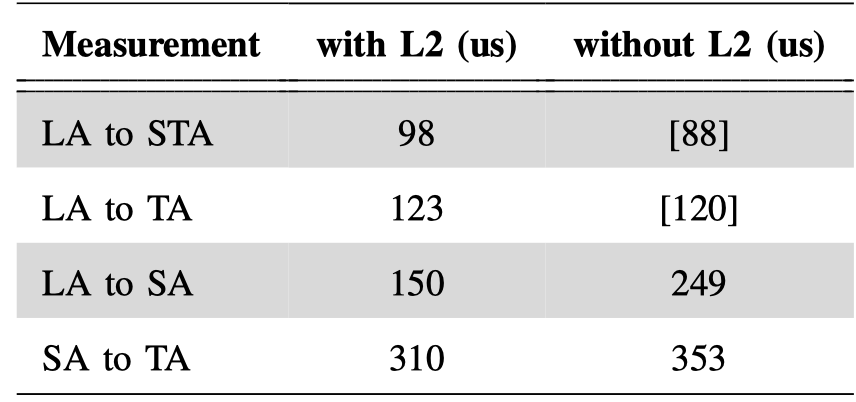
\includegraphics[scale=0.45]{Figures/trustzone/datacom.png}
    \decoRule
    \caption{SANCTUARY通讯性能}
    \label{fig:datacom}
\end{figure}

\begin{figure}
    \centering
    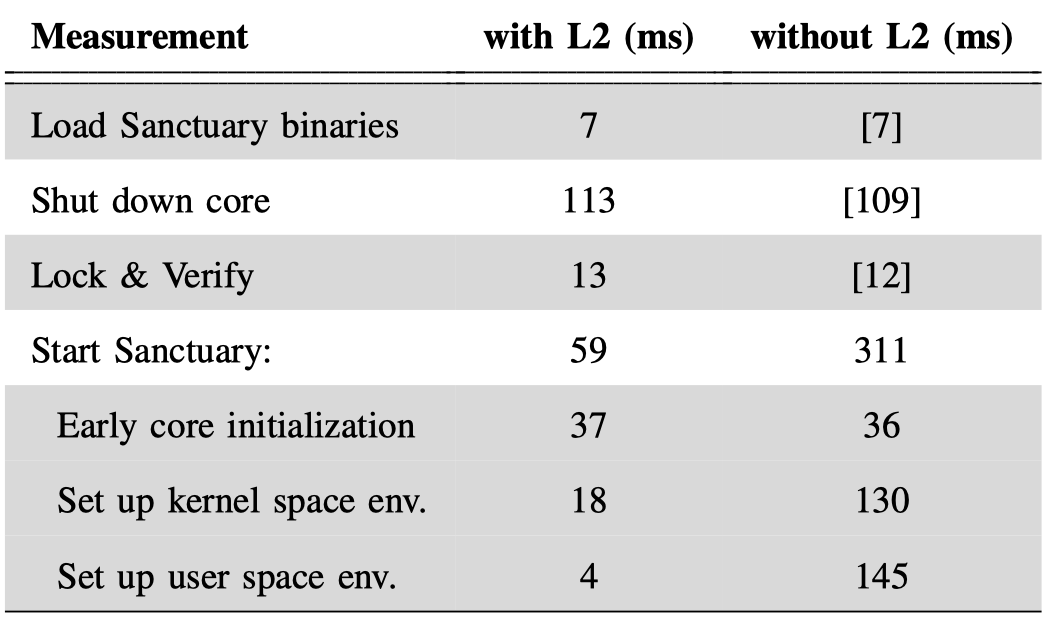
\includegraphics[scale=0.45]{Figures/trustzone/setup.png}
    \decoRule
    \caption{SANCTUARY创建性能}
    \label{fig:setup}
\end{figure}

\begin{figure}
    \centering
    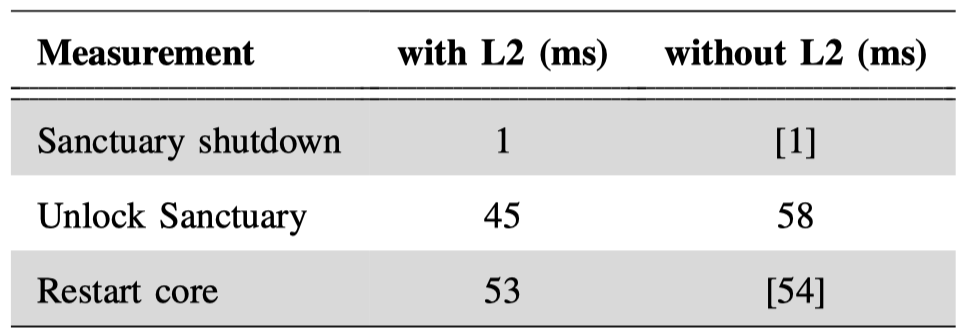
\includegraphics[scale=0.45]{Figures/trustzone/teardown.png}
    \decoRule
    \caption{SANCTUARY销毁性能}
    \label{fig:teardown}
\end{figure}

\paragraph{灵活性分析}
SANCTUARY的设计具有很好的灵活性,不仅不会更改原来的硬件结构,新增和要修改的代码也较少
可以在现有TrustZone的基础上进行直接移植,同时Sanctuary的创建和销毁灵活方便,
可以在实际场景中灵活应用。

\paragraph{可扩展性分析}
可扩展性可以分为从理论和实际两个角度来思考。
从理论和实验上来讲SANCTUARY的设计具有很好的可扩展性,任何一个Normal World的核都可以
被创建成SANCTUARY的CPU,每个Sanctuary也可容易的创建和销毁。
然而在实际终端场景中,一个核的数量终端是有限的,当Sanctuary的数量不断增加,实际可以用
的CPU就会减少,会丧失原本调度的公平性,从而使得整个系统不可用。


\subsection{不足}
\paragraph{恶意使用}
SANCTUARY自身可以有效防止数据被窃取以及获取更高权限的问题。但是其本身不能防止一些恶意
的会让其系统瘫痪的代码。如Sanctuary屏蔽了来自其他地方的中断,因此一个恶意SA可以一直不退出
导致Sanctuary不被销毁,CPU得不到释放,由多个这样的SA足以使系统瘫痪。同时恶意的LA可以通过
不断申请Sanctuary的创建大大降低CPU的利用率。

\paragraph{性能问题}
由于Sanctuary执行的App都是在唯一分配的CPU上执行代码,因此其本身不支持多线程和多核的性能优化。
在一些需要快速响应同时执行敏感数据的场景中,将带来不好的影响。如高清视频的解码。高清的视频流数据
具有版权性,往往需要保护起来,因此在接收和解码时需要放入Sanctuary中执行,而视频观看是一个响应
时间和用户体验挂钩的场景,较慢的解码速度意味着较差的用户体验。Sanctuary的单核设计让解码不能在
多个CPU同时进行,因此可能会影响用户的体验。可以思考在此基础上支持Sanctuary对多核的优化。

%----------------------------------------------------------------------------------------
%	SECTION 4
%----------------------------------------------------------------------------------------

\section{本章小结}

本章主要对TrustZone和系统SANCTUARY进行了介绍和分析,通过说明TrustZone的设计原理和不足,
引出了SANCTUARY的设计和解决方案。说明了SANCTUARY分威胁模型和安全保证。对SANCTUARY的性能
可扩展性以及灵活性进行了分析。最后讨论了SANCTUARY的不足,对于其性能问题给出了具体场景和
未来可以优化的方案。
